%%%%%%%%%%%%%%%%%%%%%%%%%%%%%%%%%%%%%%%%%
% DOCUMENTACION PASANTIA EN SONDA URUGUAY
% ING. JUAN BRAGA
% MAESTRÍA EN INGENIERÍA ELÉCTRICA, UDELAR
% JUNIO 2016
%%%%%%%%%%%%%%%%%%%%%%%%%%%%%%%%%%%%%%%%%

%----------------------------------------------------------------------------------------
%	PACKAGES AND DOCUMENT CONFIGURATIONS
%----------------------------------------------------------------------------------------

\documentclass{article}

\usepackage[version=3]{mhchem} % Package for chemical equation typesetting
\usepackage{siunitx} % Provides the \SI{}{} and \si{} command for typesetting SI units

\usepackage[spanish]{babel}
\selectlanguage{spanish}
\usepackage[utf8]{inputenc}
\usepackage{graphicx} % Required for the inclusion of images
\usepackage{natbib} % Required to change bibliography style to APA
\usepackage{amsmath} % Required for some math elements 

\usepackage[margin=0.8in]{geometry}

\setlength\parindent{0pt} % Removes all indentation from paragraphs

\renewcommand{\labelenumi}{\alph{enumi}.} % Make numbering in the enumerate environment by letter rather than number (e.g. section 6)

%\usepackage{times} % Uncomment to use the Times New Roman font

%----------------------------------------------------------------------------------------
%	DOCUMENT INFORMATION
%----------------------------------------------------------------------------------------

\title{\textbf{Desarrollo de una plataforma de procesamiento de audio en tiempo real con aplicación a seguridad urbana}\\ \textsc{Pasantía Laboral en SONDA Uruguay}\\
\large \textsc{Maestría en Ingeniería Eléctrica} del \textit{Instituto de Ingeniería Eléctrica, Facultad de Ingeniería, Universidad de la República, Uruguay.}}

\author{\textit{Ing. Juan Braga}}
\date{\today}

\begin{document}

\maketitle 

\begin{center}
\begin{tabular}{l r}
\medskip
\textsc{Período:} & \textsc{Diciembre 2015 a Marzo 2016}\\ % Date the experiment was performed
\textsc{Docente Responsable:} & \textit{Msc. Ing. Guillermo Carbajal} \\ 
\textsc{Responsable SONDA Uruguay:} & \textit{Nestor Rossi}, Gerente de Proyectos  \\
\textsc{Equipo de SONDA Uruguay:} & \textit{Ing. Florencia Lanzaro} \\ & \textit{Msc. Ing. Guillermo Carbajal} \\ 
\end{tabular}
\end{center}

%----------------------------------------------------------------------------------------
%	ABSTRACT
%----------------------------------------------------------------------------------------

\begin{abstract}
El presente informe tiene como objetivo la documentación del trabajo realizado en SONDA Uruguay en el período de Diciembre 2015 a Marzo 2016 para su aprobación en créditos de la Maestría en Ingeniería Eléctrica de la UdelaR. Se trató de un estudio del estado del arte en la aplicación de analíticas de audio a seguridad urbana y el desarrollo de una plataforma de procesamiento en tiempo real para prueba de concepto en condiciones de laboratorio. Dejando como resultado la implementación de dos analíticas particulares y su desempeño en una base de datos pública.
\end{abstract}

%----------------------------------------------------------------------------------------
%	SECTION 1
%----------------------------------------------------------------------------------------

\section{Introducción}
El monitoreo en tiempo real de actividades humanas para seguridad urbana se ha vuelto masivo en los últimos años a nivel mundial. La cantidad de sensores distribuidos por las ciudades ha crecido enormemente. Es entonces en los centros de monitoreo, donde confluyen las señales desde variados puntos de la ciudad, que surge la necesidad de automatizar los procesos de visualización y control para hacer la operativa más eficiente \citep{crocco2014audio}. El desarrollo de analíticas en tiempo real para detección automática de patrones de interés, ha captado la atención de la comunidad científica así como a empresas con fines comerciales. En este escenario es donde la empresa SONDA Uruguay motiva un proyecto de desarrollo de software de analíticas de audio y video, para el monitoreo automático en tiempo real de los espacios urbanos.  

\bigskip
En el marco del proyecto de la empresa anteriormente mencionado, se realizó una prueba de concepto sobre la implementación de analíticas de audio en tiempo real para seguridad urbana. Con este fin se realizó un estudio del estado del arte para luego seguir con el desarrollo de una plataforma de procesamiento de audio a nivel de laboratorio. 

\bigskip
En lo que sigue el documento está dividido en tres secciones. En la Sección \ref{literatura} se hace una breve revisión bibliografíca, por otro lado en la \ref{PP} se detalla sobre la plataforma de procesamiento desarrollada. En la Sección \ref{analiticas} sobre los algoritmos utilizados para la implementación de dos analíticas de audio particulares: \textit{Detección de Niveles Predefinidos de Sonido} y \textit{Detección de Sirenas}. Además en la Sección \ref{experimentos} se detalla la evaluación de desempeño y sus resultados, para dar lugar por último en la Sección \ref{concl} a una breve reflexión sobre la sinergia de la pasantía laboral y los estudios de académicos, en el marco de la Maestría de Ingeniería Eléctrica actualmente en curso.  

\subsection{Sobre SONDA Uruguay}
SONDA Uruguay es fundamentalmente una empresa de servicios, proyectos de integración de sistemas y provisión de plataformas en el campo de las tecnologías de la información. Actualmente la empresa está incorporando proyectos de I+D en el área de tratamiento de señales. Tal es el caso del proyecto de desarrollo de analíticas de audio y video en tiempo real con aplicación a seguridad urbana. En el mismo, se encuentran involucradas ocho personas, profesionales y estudiantes de Ingeniería de Sistemas y Eléctrica, que complementan la rama de computación científica con el manejo de la ingeniería de software para aplicaciones críticas de gran volumen de datos.  

%----------------------------------------------------------------------------------------
%	SECTION 2
%----------------------------------------------------------------------------------------

\section{Revisión Bibliográfica}
\label{literatura}
Si bien la investigación y desarrollo de algoritmos sobre señales de video para detección automática de eventos relevantes, son de interés para científicos y empresas hace unos años, aún hoy en día no son lo suficientemente confiables y robustos para las exigencias de aplicaciones en seguridad. Es en este escenario que los sensores de audio toman relevancia, ya sea en conjunto con el video o de forma independiente, generando el interés en la última década de la comunidad científica así como el sector comercial. 

\bigskip
En la publicación \cite{crocco2014audio} se tiene un resumen de los métodos automáticos basados en audio con aplicación a seguridad. Se especifica una taxonomía que facilita la comparación entre algoritmos y su función: \textit{Extracción de Fondo, Clasificación de Eventos, Tracking de Objetos y Análisis del Entorno}. Para cada clase se citan los trabajos más relevantes detallando los puntos fuertes y débiles. En adición se hace un análisis de expresividad de características computables a partir de audio con aplicación en las distintas etapas anteriormente mencionadas. 

\bigskip
En el marco del presente trabajo la atención se centró a los algoritmos que atacan las etapas de \textit{Extracción de Fondo} y \textit{Clasificación de Eventos} ya que son los que componen el sistema implementado. Existen diversos métodos utilizados para la \textit{Extracción de Fondo (Background Substraction en Inglés)} en audio. Los más simples se basan en medidas unidimensionales, en general basadas en la estimación de intensidad. Tal es el caso de la publicación \cite{dufaux2000automatic} para la detección automática de sonidos impulsivos tales como roturas de vidrio, tiros de pistola, explosiones, entre otros. Por otro lado los métodos basados en características multidimensionales son los de mayor robustez en escenarios complejos. En el trabajo publicado por \cite{lecomte2011abnormal} se propone un método no supervisado para la detección de eventos anormales en audio ambiente. Está basado en un \textit{One-Class SVM} para modelar la distribución del sonido normal en un ambiente y extracción de características basadas en un banco de filtros. Además introduce un método para generar una base de datos de sonidos basada en audio reales.
 
\bigskip 
En cuanto a la clasificación de eventos en audio, usualmente se resuelve con un enfoque de clasificación supervisada. En primer lugar características son computadas a partir de las muestras de audio etiquetadas, permitiendo aprender un clasificador especifico en base a un conjunto acotado de muestras, de manera \textit{off-line}. A este primera etapa se la suele llamar de \textit{Entrenamiento}. Luego se da paso a la evaluación del desempeño del clasificador entrenado, con nuevas muestras de audio no utilizadas en la etapa anterior. En el libro \textit{Introduction to Audio Content Analysis} \citep{Lerch:2012:IAC:2392638} el Capítulo 3 está dedicado a las características de tiempo corto o instantáneas. Son denominadas así las que se computan en un entorno temporal de la muestra actual donde la naturaleza de la señal se puede suponer estacionaria. Se encuentran divididas en 4 clases para facilidad de comprensión: \textit{Propiedades Estadísticas, Forma Espectral, Propiedades de la Señal y Propiedades de Intensidad}. Siendo un buen manual para consulta rápida de las características más utilizadas. En el siguiente Capítulo del mismo libro se detalla sobre la medida de intensidad en señales de audio, comienza desambigüando los términos \textit{Sonoridad (Loudness en Inglés)} e \textit{Intensidad}, haciendo un paralelismo con las dinámicas en música y definiendo las medidas de intensidad más comunes.
\bigskip

Debido al interés por esta rama de investigación, en el último tiempo se han hecho disponibles \textit{challenges} y bases de datos de acceso público de sonidos generados a partir de ambiente urbanos. Tal es el caso de \textit{TUT Database} creada para la clasificación de escenarios acústicos y detección de eventos de interés en ambientes urbanos \citep{mesaros2016tut}. Vale mencionar además, la base de datos que se usa para evaluación de desempeño en el presente trabajo es la denominada \textit{Urban Sound Dataset} \citep{Salamon:UrbanSound:ACMMM:14} en particular se trabaja con la \textit{UrbanSound8K}, donde los fragmentos de audio contienen sonidos particulares predominantes. 

%----------------------------------------------------------------------------------------
%	SECTION 2
%----------------------------------------------------------------------------------------

\section{Plataforma de Procesamiento}
\label{PP}
Los sensores para Seguridad Urbana (en particular las cámaras de video y micrófonos) son diseñados para trabajar en tiempo real, transmitiendo a través de una red IP los datos adquiridos, a una central donde se realiza el monitoreo y la toma de decisiones. Es en este escenario donde los algoritmos de procesamiento de audio se encuentran embebidos y los tiempos de procesamiento no deben exceder la cadencia de disponibilidad de datos.

\bigskip
La plataforma de procesamiento, se puede dividir en dos grandes bloques: por un lado el de genereración de datos de audio y comunicaciones, y por otro la adquisición desde la red y procesamiento para la toma de decisiones, como se observa en la Figura \ref{fig:plataforma_procesamiento}.
\bigskip

Del lado de la generación de los datos de audio el tipo de micrófono (patrón polar, sensibilidad, etc.) y el codec (frecuencia de muestreo, bitdepth, etc.) definen la información sonora que se extrae del escenario monitoreado. El tipo de análisis que se pueda hacer va a depender de las anteriores características del sistema. En particular el micrófono que se utiliza para la prueba de concepto es activo y omnidireccional, características deseables en aplicaciones de seguridad debido a la alta sensiblidad y la \textit{escucha} de la escena completa. En adición el manejo de \textit{streaming} así como los \textit{codecs} de audio se hace por medio del software \textit{FFmpeg} \citep{bellard2012ffmpeg}. Además para utilización en ambiente de laboratorio se implementó el streaming de archivos para trabajar con audios controlados, como se puede observar en el recuadro de la izquierda en la Figura \ref{fig:plataforma_procesamiento}. 
\bigskip

Por otro lado el módulo de adquisición hace disponible las muestras de audio, en ventanas de largo configurable según los requerimientos del algoritmo. El análisis se hace ventana a ventana (frame by frame en la literatura) y en el caso particular de \textit{Detección de Sirenas} (sección: \ref{deteccion de sirenas}), se utiliza una estrategia de integración temporal para aumentar la robustez a falsas alarmas, debidas al análisis local ventana a ventana. La implementación de las analíticas en tiempo real se realiza utilizando el lenguaje de programación \textit{Python}, con librerías de computación científica como \textit{SciPy} \citep{jones2001open}, \textit{Librosa} \citep{mcfee2015librosa} para procesamiento de audio y \textit{Sci-kit Learn} para algoritmos de machine learning \citep{pedregosa2011scikit}. En adición, la herramienta \textit{Weka} \citep{hall2009weka} se utiliza para evaluación de desempeño.  


\begin{figure}[h]
\begin{center}
\includegraphics[width=0.65\textwidth]{plataforma_procesamiento} 
\caption{Esquema de la plataforma de procesamiento. A la izquierda el bloque de generación y comunicaciones, a la derecha el de adquisición y procesamiento.}
\label{fig:plataforma_procesamiento}
\end{center}
\end{figure}

%----------------------------------------------------------------------------------------
%	SECTION 3
%----------------------------------------------------------------------------------------

\section{Analíticas}
\label{analiticas}
Las analíticas son el núcleo de procesamiento de audio que transforman los datos de entrada en una decisión para generar una alarma. Tienen el objetivo de alertar ante hechos predefinidos que puedan estar asociados a actividades vandálicas. En esta sección se describe sobre dos analíticas desarrolladas en la primer etapa del proyecto de desarrollo del software de analíticas de audio. 

\subsection{Analítica de Detección de Niveles Predefinidos de Sonido}
Tiene como objetivo alertar la presencia de momentos de alto nivel sonoro o ausencia del mismo. Se hace una estimación de la energía, de la señal de entrada, frame a frame y se umbraliza para generar alertas en niveles energéticos predefinidos por el usuario.

\subsubsection{Medidas de energía}
Se utilizan dos estimaciones de energía para detección de cambios energéticos de distinta naturaleza, por un lado cambios sostenidos en el tiempo y por otro lado los impulsivos.

\subsubsection*{RMS}
Se utiliza para estimar la energía promedio de la ventana temporal. La ecuación para una ventana de largo N es de la siguiente forma \cite[Chapter~4]{Lerch:2012:IAC:2392638}:
\begin{equation}
RMS = \sqrt{\frac{1}{N}\sum_{n=1}^{N} x[n]^2}
\end{equation}

\subsubsection*{Envolvente de pico}
Se utiliza para detectar eventos energéticos impulsivos que pueden ser disimulados por el promediado del valor RMS. El cálculo para una ventana de largo N se realiza de la siguiente forma \cite[Chapter~4]{Lerch:2012:IAC:2392638}:
\begin{equation}
PICO = max(x[n]) \quad \forall n \in 1..N 
\end{equation}

\subsubsection{Detección de altos niveles sonoros}
Para esta analítica se utiliza una estrategia de doble umbral sobre las estimaciones de energía detalladas anteriormente. En primer lugar se aplica al valor RMS de la ventana temporal, siendo útil frente a cambios energéticos sostenidos en el tiempo. Por otro lado se umbraliza el valor de pico, para detectar eventos impulsivos que no sean detectables en el promediado del RMS.

\subsubsection{Detección de bajos niveles sonoros}
Para la umbralización inferior sólo se trabaja con el valor RMS.

\subsection{Analítica de Detección de Sirenas}
\label{deteccion de sirenas}
Tiene como objetivo alertar frente a al presencia de una sirena en el audio de análisis. Para esta analítica se utiliza una estrategia de reconocimiento de patrones con el entrenamiento de clasificadores. Se resuelve con el enfoque clásico de reconocimiento de sonidos particulares para Seguridad Urbana de dos etapas, \cite{lecomte2011abnormal}:
\begin{enumerate}
\begin{item}
Detección de eventos anómalos
\end{item}
\begin{item}
Reconocimiento de los eventos anómalos detectados
\end{item}
\end{enumerate}

Se trata de dos clasificadores anidados con una etapa de integración temporal intermedia. En la primer etapa, con un modelado no supervisado del ruido ambiente se detectan anormalidades en el audio, si existieron los suficientes eventos anómalos según la integración temporal, se pasa a la tercer y última etapa, donde se clasifica en sirena o no. Se observa un esquema de lo dicho anteriormente en la Figura \ref{fig:deteccion_sirenas}. 
 
\begin{figure}[h]
\begin{center}
\includegraphics[width=0.65\textwidth]{deteccion_sirenas} 
\caption{Esquema de la analítica de detección de sirenas. Se observa una primer etapa de substracción de fondo y posterior clasificación en sirena o no.}
\label{fig:deteccion_sirenas}
\end{center}
\end{figure}

\subsubsection{Substractor de Fondo}
En aplicaciones de Seguridad Urbana, se utilizan algoritmos de substracción de fondo (en la literatura \textit{Background Substraction}, \cite{crocco2014audio}) como una primer etapa de análisis y conceptualización de la señal de entrada. En otras palabras estos algoritmos modelan los patrones que dominan el ambiente y detectan anormalidades.
\bigskip 

El modelado del ruido ambiente con un enfoque supervisado tiene la dificultad de la generación de una base de datos que resuma y caracterice la infinidad de posibilidades que existen en un entorno urbano. Por esta razón se optó por un enfoque de clase unitaria utilizando One-Class SVM (\cite{rabaoui2008one}, \citep{lecomte2011abnormal}).

\subsubsection*{Extracción de Características}
Teniendo en cuenta que no se conoce nada a priori sobre el ruido ambiente y además el sistema está basado en un análisis por ventana (en la literatura frame by frame), para la extracción de características se utiliza el enfoque genérico de un banco de filtros lineal, para extracción de la energía en bandas de frequencia de la transformada de Fourier (Fourier-based linear filterbank \citep{lecomte2011abnormal}).

\subsubsection*{Entrenamiento y Clasificación}
El entrenamiento se realiza en tiempo real, con fragmentos del propio ruido ambiente en donde el sistema se encuentra funcionando. Permite independencia de una base de datos para entrenamiento y robustez frente a cambios naturales en el escenario de análisis, como son la noche y el día por ejemplo. 
\bigskip

El largo del fragmento es variable permitiendo adaptarse a escenarios complejos, sacrificando costo computacional. Se utiliza un clasificador One-Class SVM que detecta en cada ventana de entrada si pertenece o no al modelo de fondo generado en el One-Class SVM.

\subsubsection{Integración temporal}

Previo a la etapa de clasificación de sirena o no, se utiliza un esquema de integración temporal. Aproximadamente audios de \textit{4 segundos} son entregados a la segunda etapa de esta analítica para su clasificación.  A partir de una medida de distancia para decidir si continuar o descartar las muestras de audio.

\bigskip
Se integran ventanas adyacentes donde las no pertenecientes al fondo se las etiqueta con un $1$ y $0$ a las contrarias. Luego ese vector es comparado con uno de igual dimensión y todas las entradas de valor $1$. Mediante la distancia binaria de Huffman, con un umbral parametrizable, se define si el fragmento de audio en cuestión pasa a la siguiente etapa de clasificación, observar Figura \ref{fig:integracion_temporal}.  

\begin{figure}[h]
\begin{center}
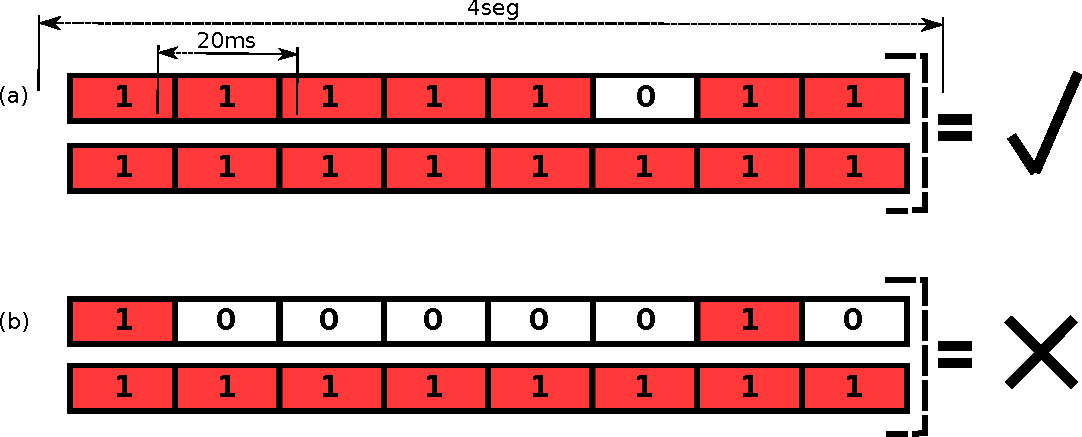
\includegraphics[width=0.65\textwidth]{integracion_temporal} 
\caption{Esquema de la integración temporal de ventanas adyacentes en un fragmento de audio mayor, se ejemplifica con dos valores particulares en segundos. En rojo los audios detectados como no fondo, en blanco los que pertenecen al fondo según el substractor de fondo. En (a) se observa un audio que pasa a la segunda etapa de clasificación, en (b) caso contrario.}
\label{fig:integracion_temporal}
\end{center}
\end{figure}
 
\subsubsection{Clasificación Sirena}
\label{onesvmsirena}
La última etapa es un clasificador One-Class SVM que decide si el evento anómalo sostenido en el tiempo, según las etapas anteriores, clasifica como sirena o no. Teniendo en cuenta que en el caso de esta analítica particular, \textit{Detección de Sirenas}, el problema se transforma en uno de clase unitaria, se decidió trabajar en esta etapa con un clasificador \textit{One-Class SVM}. 


\subsubsection*{Extracción de Características}
Se utilizan al igual que en la publicación \cite{Salamon:UrbanSound:ACMMM:14} los primeros 25 coeficientes MFCC (Mel-Frequency Cepstral Coeficients), calculados sobre un banco de filtros Mel de 40 bandas, generado con ventanas temporales de 20ms, 50\% de solapamiento y enventanado hamming. Lo anterior se computa sobre el audio completo que sale de la integración temporal (en la Figura \ref{fig:integracion_temporal} se ejemplifica con 4 segundos de audio) y se aplican estadísticas para resumir a un vector de 275 características: máximo, mínimo, media, mediana, varianza, skewness, kurtosis y media y varianza de la primer y segunda derivada de los coeficientes Mel a lo largo del tiempo.

\subsubsection*{Entrenamiento y Clasificación}
Para el entrenamiento se utilizó un enfoque de clase unitaria utilizando One-Class SVM. Como base de datos para entrenamiento y test se utilizó la UrbanSound dataset publicada en \cite{Salamon:UrbanSound:ACMMM:14}. 

%----------------------------------------------------------------------------------------
%	SECTION 4
%----------------------------------------------------------------------------------------

\section{Experimentos}
\label{experimentos}

En esta sección se detallan los experimentos realizados durante la prueba de concepto. La sección está dividida en dos partes. En primer lugar, se realizan tres experimentos para determinar el poder de separación de características basadas en los clásicos \textit{Mel Frequency Cepstral Coefficients} \citep{davis1980comparison}, aplicado a sonidos urbanos de la base de datos de acceso público \textit{UrbanSound8K} \citep{Salamon:UrbanSound:ACMMM:14}. El primero de los experimentos sigue los lineamientos de la publicación \citep{Salamon:UrbanSound:ACMMM:14} a modo de comparación y como un mojón para los siguientes resultados. En el segundo, se modifica la frecuencia de muestreo de los audios de \textit{UrbanSound8K} de \textit{44100Hz} a \textit{8000Hz} para simular las condiciones en la que trabaja la plataforma de procesamiento, sin variar la extracción de características. Por último se evalúa el desempeño, también a tasa de muestreo \textit{8000Hz} pero disminuyendo la cantidad de bandas \textit{Mel} en la extracción de características. 

\bigskip
Por otra parte, la segunda sección está centrada en la evaluación de la plataforma completa para ambas analíticas funcionando en tiempo real. Se describe la experiencia realizada en ambiente de laboratorio donde de forma cualitativa se evaluó el desempeño.

\subsection{Evaluación del poder de separación en la base \textit{UrbanSound8K}}
\label{poderseparacion}
El objetivo de la presente sección es evaluar el poder de separación de características basadas en \textit{MFCC} \citep{davis1980comparison} aplicado a la problemática de sonidos urbanos. Estos coeficientes como características de un sistema de reconocimiento automático del hablante han demostrado tener de los mejores desempeños \citep[Capítulo 14]{quatieri2002discrete}. A partir de ahí han sido utilizados en diversas problemáticas de clasificación que no involucran señales de voz hablada, con buenos resultados también como es el caso de reconocimiento de instrumentos \citep[Capítulo 6]{klapuri2007signal}. Su fortaleza radica en la incorporación del modelado psicoacústico de la audición humana mediante un banco de filtros basados en la escala \textit{Mel} \citep{stevens1937scale} y la decorrleación que presentan los datos en el dominio de las \textit{quefrencys}, dado por la Transformada Coseno. Son un buen descriptor para la extracción de aspectos tímbricos de la señal.

\bigskip
Para evitar el bías que pueda existir entre las características computadas y algún clasificador particular, las pruebas se hacen con más de un clasificador clásico, utilizando el software \textit{Weka} \citep{hall2009weka}.

\bigskip
Se trabaja con la base de datos de acceso público llamada \textit{UrbanSound8K} \citep{Salamon:UrbanSound:ACMMM:14}. Está organizada en 10 clases de sonidos urbanos: \textit{Calle, Niños, Ladrido de Perro, Aire Acondicionado, Perforación, Martillo Neumático, Motor, Sirena, Bocina de Auto y Disparo}. Está constituida por audios reales de ambientes urbanos. A partir de los cuales se generan clips, de duración máxima 4 segundos, donde predomina alguna de las anteriores clases. Para evitar redundancia en la etapa de test, la base viene con 10 \textit{folds} generados de forma que no existan clips del mismo audio original en dos \textit{folds} distintos.

\subsubsection{Extracción de características}
\label{extcar}
En los dos primeros experimentos de esta Sección \ref{poderseparacion}, se utilizan al igual que en la publicación \cite{Salamon:UrbanSound:ACMMM:14}, los primeros 25 coeficientes MFCC (Mel-Frequency Cepstral Coeficients), calculados sobre un banco de filtros Mel de 40 bandas. Los coeficientes son generados con ventanas temporales de 20ms, 50\% de solapamiento y enventanado hamming a lo largo de los 4 segundos de audio. Posteriormente se aplican estadísticas a lo largo del tiempo para resumir los coeficientes a un vector de 275 características: máximo, mínimo, media, mediana, varianza, skewness, kurtosis y media y varianza de la primer y segunda derivada. En la Figura \ref{fig:bandasmel1} se puede observar la disposición del banco de filtros \textit{Mel} para el cálculo de los coeficientes para ambos casos (con tasa de muestreo de \textit{44.1Khz} y \textit{8Khz}), para esto se utiliza el módulo de \textit{Python} detallado en la publicación \cite{mcfee2015librosa}. Vale resaltar que si bien los parámetros para el cálculo de coeficientes en ambas frecuencias de muestreo son los mismos, la resolución del banco de filtros en el rango de \textit{0 a 4Khz}, para el caso de \textit{8Khz} es mayor que para \textit{44.1KHz} como se puede observar en la Figura \ref{fig:bandasmel2}.

\begin{figure}[h]
\begin{center}
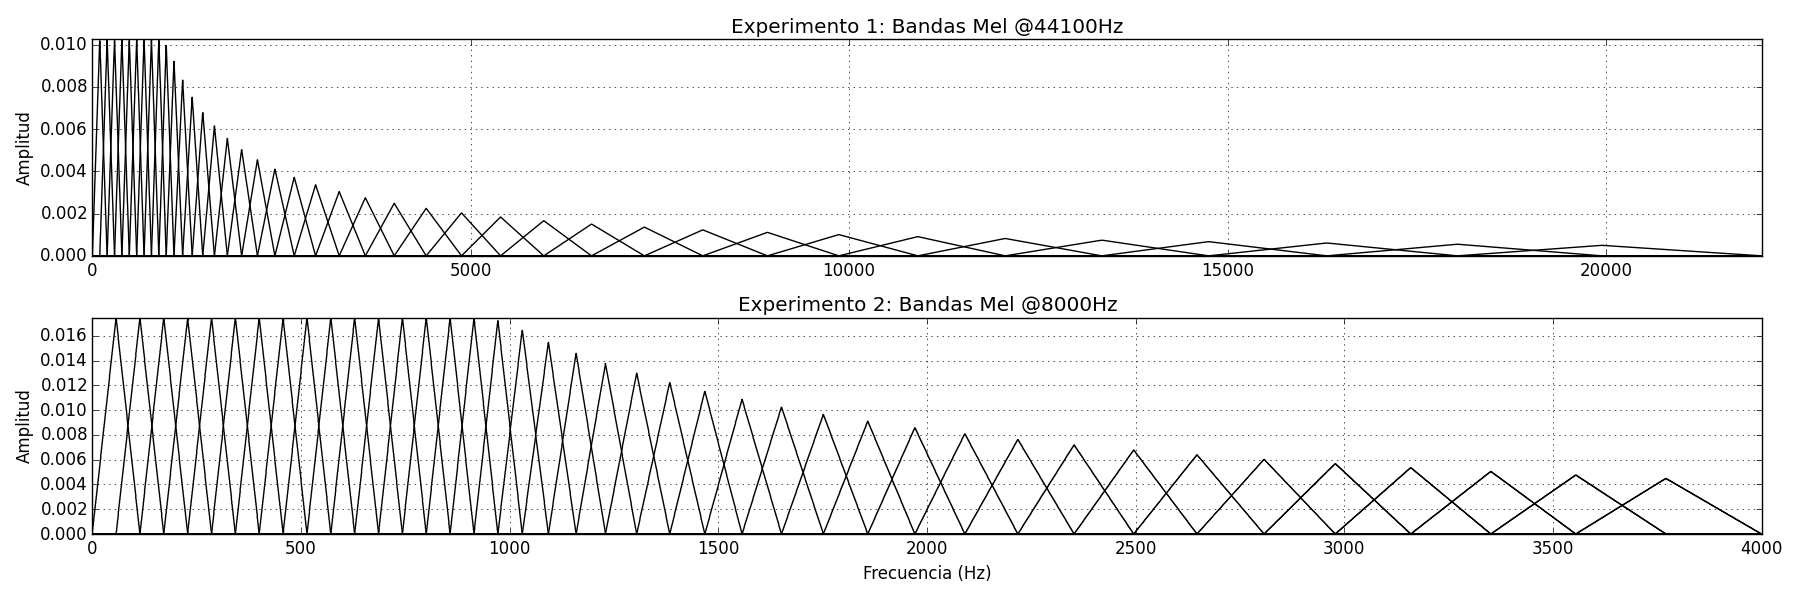
\includegraphics[width=1\textwidth]{bandasmel1} 
\caption{Disposición del filtro de bandas \textit{Mel} para la extracción de características con 40 bandas de los Experimentos 1 y 2. }
\label{fig:bandasmel1}
\end{center}
\end{figure}

De lo dicho anteriormente el tercer experimento de la presente sección evalúa el poder de separación en los datos muestreados a \textit{8Khz}, extrayendo los \textit{MFCC} con 25 bandas de manera que la resolución en el rango que va desde \textit{0 a 4KHz} sea similar. Esto se observa en la Figura \ref{fig:bandasmel2}.

\begin{figure}[h]
\begin{center}
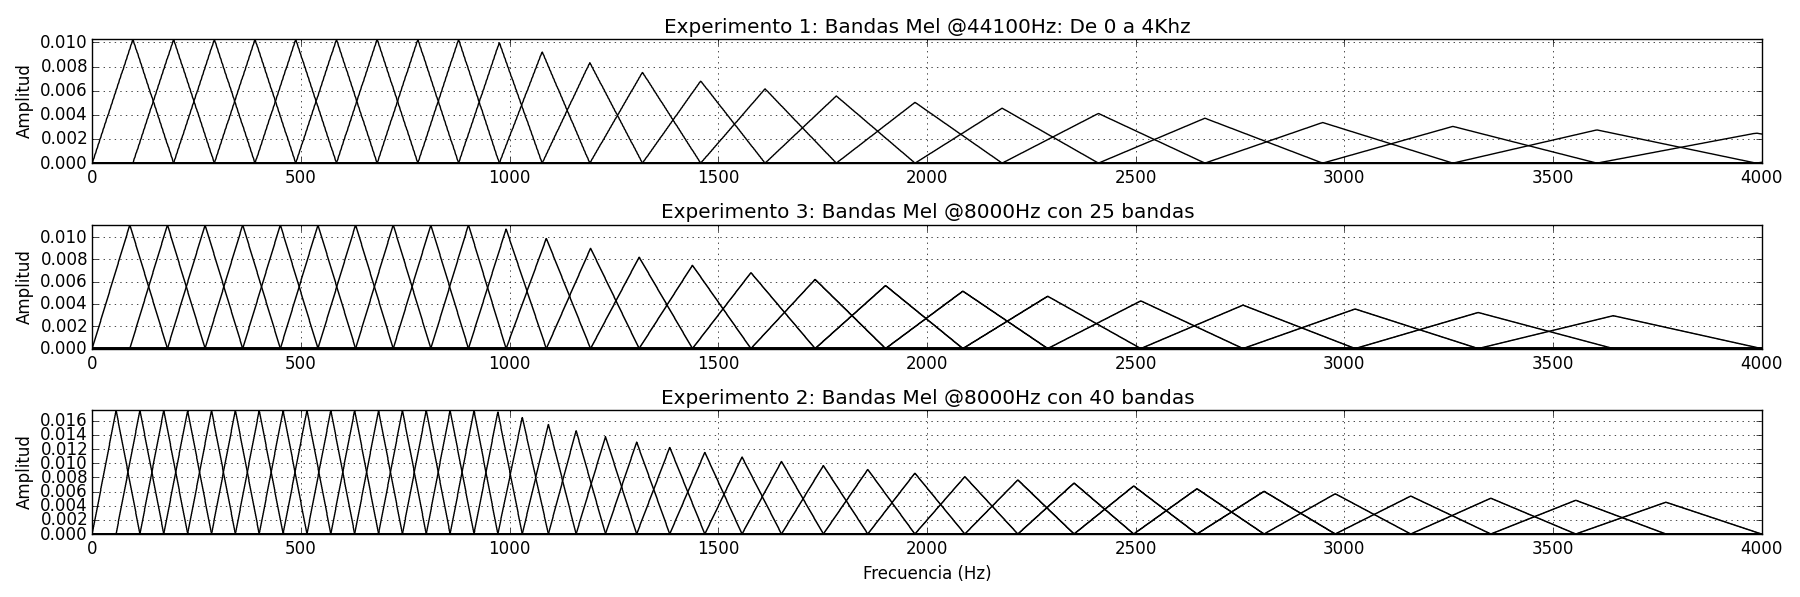
\includegraphics[width=1\textwidth]{bandasmel2} 
\caption{Disposición del filtro de bandas \textit{Mel} en el rango \textit{0 a 4Khz} para la extracción de características con 40 bandas de los Experimentos 1 y 2 y con 25 bandas para el Experimento 3.}
\label{fig:bandasmel2}
\end{center}
\end{figure}

\subsubsection{Resultados y Discusión}

En la Figura \ref{fig:boxplots} se detallan los resultados de los experimentos representados como \textit{Boxplots} (por su denominación en Inglés). Todos los experimentos fueron realizados con \textit{10-fold validation}, utilizando la división realizada por los autores de la base, como fue detallada al principio de esta Sección \ref{poderseparacion}. La medida de desempeño utilizada es el \textit{Accuracy}: proporción entre número de elementos bien clasificados y el total. 


\begin{equation}
\textit{Accuracy} = \frac{VP + VN}{\textit{Total}}
\end{equation}


Para evitar el bías que pueda existir entre el espacio de características y algún clasificador particular la clasificación se realizó para el Experimento 1 con cuatro clasificadores clásicos:

\begin{itemize}
  \item \textit{Support Vector Machines (SMO en Weka)}: con núcleo \textit{RBF} y parámetros por defecto.
  \item \textit{Random Forest (RandomForest en Weka)}: con 500 árboles.
  \item \textit{K-Nearest Neighbors (IBk en Weka)}: con $k=5$.
  \item \textit{Decision Trees (J48 en Weka)}: con parámetros por defecto.
\end{itemize}
Dado la superioridad de los resultados para los dos primeros clasificadores, el resto de los experimentos se realizó solo con \textit{Support Vector Machines} y \textit{Random Forest}. 

\begin{figure}[h]
\begin{center}
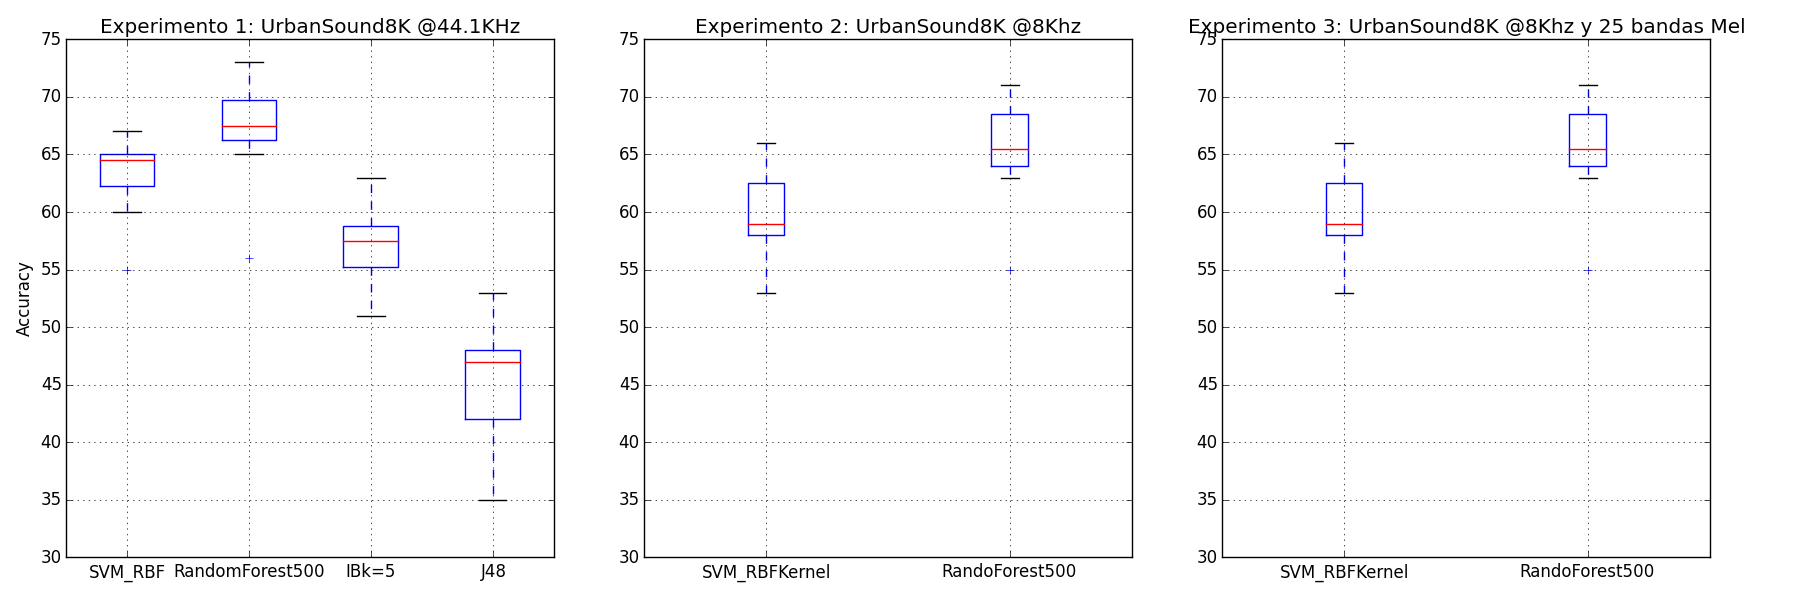
\includegraphics[width=1\textwidth]{boxplots} 
\caption{Desempeño en la clasificación con \textit{UrbanSound8K}. De izquierda a derecha respectivamente se puede observar: \textbf{(a)} Poder de clasificación siguiendo los lineamientos de la publicación \citep{Salamon:UrbanSound:ACMMM:14}, \textbf{(b)} Poder de clasificación (con los clasificadores de mejor desempeño en \textbf{(a)}) para la base de datos submuestrada a \textit{8Khz} con 40 bandas \textit{Mel}, \textbf{(c)} Poder de clasificación para la base de datos submuestreada a \textit{8Khz} con 25 bandas \textit{Mel}}
\label{fig:boxplots}
\end{center}
\end{figure}

En primer lugar vale resaltar que los resultados que se obtienen siguiendo los lineamientos de la publicación de \citep{Salamon:UrbanSound:ACMMM:14} están por debajo a los reportados. Los clasificadores \textit{Support Vector Machines} y \textit{Random Forest} de mejor desempeño en el Experimento 1, si bien no alcanzan, tampoco se alejan tanto del valor reportado en \cite{Salamon:UrbanSound:ACMMM:14}. La diferencia en desempeño a priori es multicausal. Existen elementos como el pre-procesamiento del audio, la normalización o escalamiento de los datos que podrían mejorar los resultados. De cualquier manera no es cometido del presente trabajo alcanzar con exactitud los resultados detallados en la publicación. Simplemente tomar el valor como referencia para comparación con los siguientes experimentos en los que se modifica la naturaleza de la base de datos.

\bigskip
Por otro lado el submuestreo de los datos si bien fueron realizados siguiendo las recomendaciones del \textit{Teorema de Nyquist} para los Experimentos 2 y 3, existe pérdida de información de alta frecuencia que puede ser útil a priori para la clasificación. Esto se comprueba en la disminución del \textit{Accuracy} que se observa en la Figura \ref{experimentos}, para ambos clasificadores. Se comprueba entonces la disminución del poder de clasificación con frecuencia de muestreo menor, como se podía esperar a priori. De cualquier manera la tasa de muestreo debe ser \textit{8Khz}, ya que es requerimiento del sistema.  

\bigskip
Por último en el Experimento 3, la disminución de bandas \textit{Mel} de manera que la resolución en el rango de \textit{0 a 4Khz} sea similar a el caso de \textit{44.1Khz} como se adelantó en la Sección \ref{extcar}, mantiene el desempeño comparado con el Experimento 2. Se puede decir entonces que para el presente trabajo no es necesario trabajar con la resolución de 40 bandas \textit{Mel}. 

\subsection{Evaluación de las analíticas}

El cometido principal de las pruebas de la presente sección es la validación del funcionamiento de ambas analíticas en tiempo real, en conjunto con la plataforma de procesamiento implementada. Para esto se condujeron dos pruebas en condiciones de laboratorio, cada una asociada a una analítica distinta. La evaluación de desempeño se realizó de forma cualitativa, siendo objetivo la validación del funcionamiento en tiempo real. 

\bigskip
Como se detalla en la Sección \ref{PP} la cadencia con la que los frames se hacen disponibles a la analítica determina el tiempo máximo de procesamiento para funcionamiento sin pérdida de frames. En condiciones de laboratorio se probó la plataforma implementada para ambas analíticas en tiempo real, en una computadora con procesador \textit{i7-3770K @ 3.50GHz}, \textit{64-bits} y \textit{8GB de RAM}. Para la analítica \textit{Detección de Niveles Predefinidos de Sonido} su funcionamiento fue sin pérdida de frames mientras que en la de \textit{Detección de Sirenas}, se pierden frames en los momentos que genera el modelo de fondo para el \textit{Background Substraction}.       

   
\subsubsection{Analítica de Sirena}

En esta sección evalúa el clasificador que toma la decisión final en la analítica de \textit{Detección de Sirenas} (detallado en la Sección \ref{onesvmsirena}). Si bien la evaluación de desempeño en esta parte se realiza también con la base de datos de acceso público \textit{UrbanSound8K} \citep{Salamon:UrbanSound:ACMMM:14}, el problema es ahora enfocado como uno de clase unitaria desde el punto de vista de clasificación. La decisión que se toma es la de si es sirena o no, utilizando el algoritmo \textit{One-Class SVM} (ver Sección \ref{deteccion de sirenas}). Por lo que para la etapa de entrenamiento se utilizan solo audios de sirena, seleccionados previamente de los 9 \textit{folds} correpondientes. La etapa de test se realiza con el \textit{fold} restante que no se usó en la etapa de entrenamiento, con la totalidad de las clases. Desembocando en un conjunto de test desbalanceado donde la clase negativa es mas numerosa que la positiva.

\bigskip
La extracción de características, al igual que en los experimentos de la Sección \ref{extcar}, se calcula como: los primeros 25 coeficientes MFCC (Mel-Frequency Cepstral Coeficients), calculados sobre un banco de filtros Mel de 40 bandas. Los coeficientes son generados con ventanas temporales de 20ms, 50\% de solapamiento y enventanado hamming a lo largo de los 4 segundos de audio. A los cuales se aplican estadísticas a lo largo del tiempo para resumirlos a un vector de dimensión 275: máximo, mínimo, media, mediana, varianza, skewness, kurtosis y media y varianza de la primer y segunda derivada.

\bigskip
Para la evaluación de desempeño se ajustó el clasificador de forma que el algoritmo pierda la menor cantidad de sirenas posibles. Este criterio se justificaría desde el punto de vista de la aplicación, si se quiere obtener un sistema en el que se pasen por alto la menor cantidad de sirenas, a costa de mayor cantida de falsas alarmas. En otras palabras los parámetros elegidos responden a un punto de funcionamiento en el que el \textit{Recall} es alto, sacrificando \textit{Precision} (ambos términos por su denominación en Inglés). 

\bigskip A continuación se muestra la evaluación de desempeño de este clasificador, ultima etapa de la analítica \textit{Detección de Sirenas}. El experimento se realizó en el punto de funcionamiento que cumple cualitativamente con el criterio mencionado anteriormente. Se muestra entonces en forma de \textit{boxplot}: \textit{Accuracy}, \textit{Precision} y \textit{Recall} en la Figura \ref{fig:boxplots_one}. Los indicadores \textit{Precision} y \textit{Recall} fueron calculados compensando el desbalance entre la clase positiva y la clase negativa, como se observa en la Ecuación \ref{eq:precrecalpha}.

\begin{equation}
\label{eq:precrecalpha}
\textit{Precision} = \frac{\alpha * TP}{\alpha * TP + FP} \quad
\textit{Recall} = \frac{\alpha * TP}{\alpha * TP + FN} \quad
\textrm{con} \quad \alpha = \frac{\textit{Clase Negativa}}{\textit{Clase Positiva}} 
\end{equation}


 
\begin{figure}[h]
\begin{center}
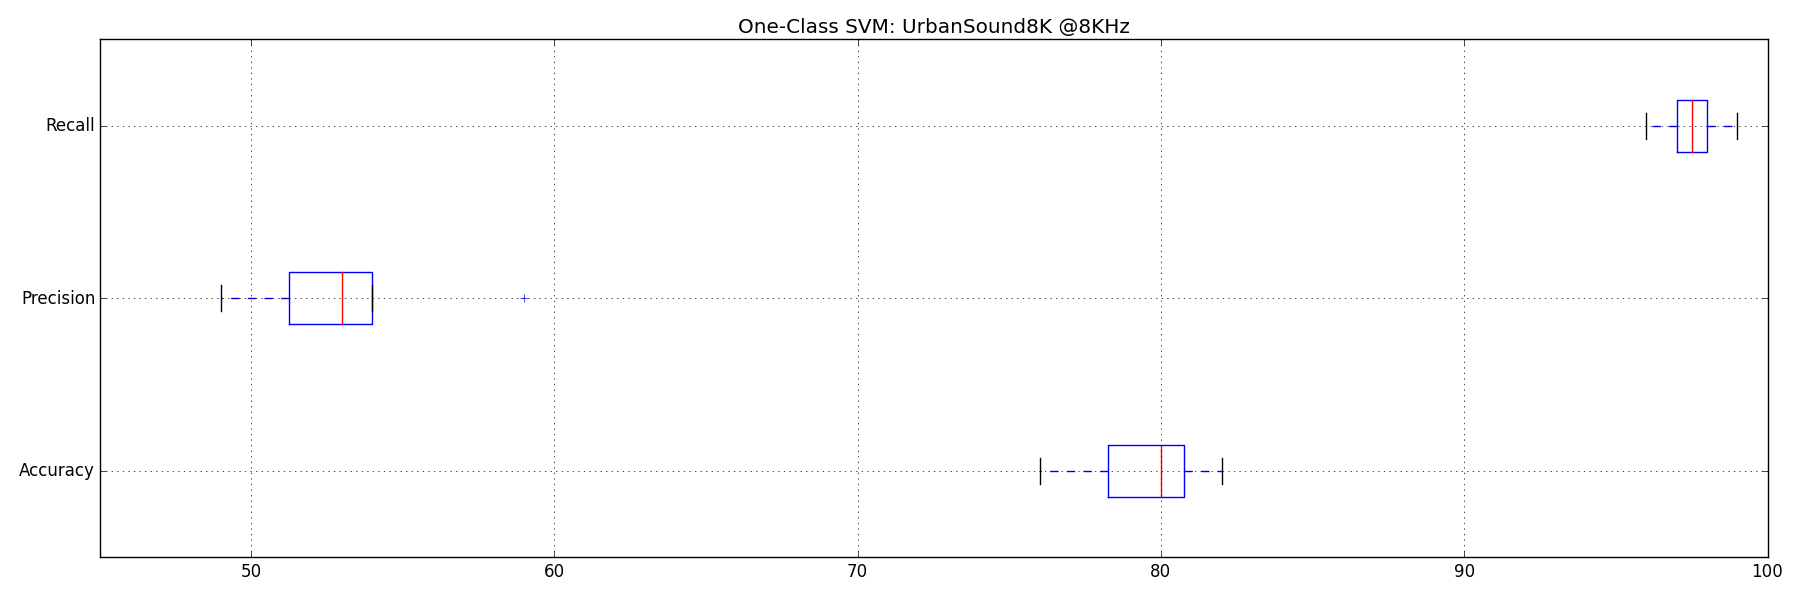
\includegraphics[width=1\textwidth]{boxplots_one} 
\caption{Desempeño en la clasificación de la última etapa en la analítica de \textit{Detección de Sirenas}}
\label{fig:boxplots_one}
\end{center}
\end{figure}

%----------------------------------------------------------------------------------------
%	SECTION 6
%----------------------------------------------------------------------------------------

\section{Conclusiones Generales sobre la Pasantía}
\label{concl}
La pasantía laboral generó sinergia de mis estudios académicos y mi trabajo en el sector privado. El desarrollo de analíticas de audio requiere de habilidades en procesamiento de audio que están vinculadas directamente con mi tema de tesis. Además se procedió con metodologías y herramientas aprendidas en la Maestría en Ingeniería Eléctrica de la Facultad de Ingeniería, como la realización de una revisión bibliográfica de publicaciones científicas para dominar el estado del arte, y la utilización de herramientas vistas en cursos de la maestría.




%----------------------------------------------------------------------------------------
%	BIBLIOGRAPHY
%----------------------------------------------------------------------------------------


\newpage
\bibliographystyle{apalike}
\bibliography{sample}

%----------------------------------------------------------------------------------------
\end{document}
